\section{Linear Model Identification}
The linearized model derived previously can be used for model parameter
identification. The idea is to identify the lumped linear model parameters and
then use this information to arrive at the estimates for the relevant parameters
for prediction/aging-factor estimation purposes.

The test-cell data used for the identification of the linear model includes measurements of all the inputs, output and the first two states of the
model. Thus, for model parameter estimation, the following regression form that
combines equations~(\ref{eqn::I2S_regression_form}) and
(\ref{eqn::I2O_regression_form}) can be used:
\begin{align}\label{eqn::regression_form}
    \bm{\frac{d^4 x_1}{dt^4}\\
        \frac{d^4 x_2}{dt^4}\\
        \frac{d^4 y_1}{dt^4}}
    &= \bm{\pmb \phi_D(x_1)
            & \pmb \phi_{N_1}
            & \pmb 0
            & \pmb 0\\
            \pmb \phi_D(x_2)
            & \pmb 0
            & \pmb \phi_{N_2}
            &\pmb 0\\
            \pmb \phi_D(y_1)
            & \pmb 0
            & \pmb 0
            & \pmb \phi_{N_y}}
        \bm{\pmb \theta_D \\ \pmb \theta_{N_1} \\ \pmb \theta_{N_2}\\ \pmb \theta_{N_y}}
\end{align}

The higher-order derivatives are computed using Savitzky-Golay FIR filter
(\cite{schafer2011savitzky}) with break frequency around $0.3\, Hz$, with any
lag being compensated for by shifting and truncating the data. The choice of
break frequency is based on the frequency response of the test-cell data.
The model comprises 45 parameters that need to be estimated, derived
from three independent measurement channels. Linear least-squares method
would result in the minimum variance and unbiased parameter estimates for this
model structure (\cite{lennart1999system}). A nonlinear inequality constraint
based on Routh-Hurwitz criterion is used to ensure the stability of the common
denominator polynomial.
%===============================================================================
\subsection{Model structure validation and parameter estimation}

\begin{figure}[h]
    \centering
    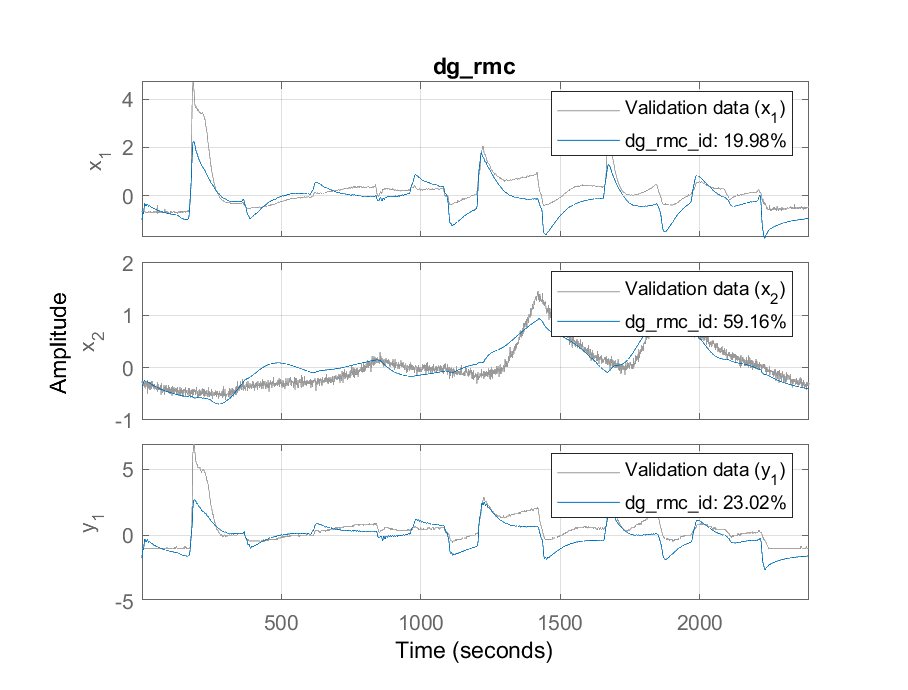
\includegraphics[width=0.7\textwidth]{Part3/figs/4_figs/dg_valid.eps}
    \caption{Comparison of the identified model with the normalized RMC test data for degreened catalyst}
    \label{fig:dg_comp}
\end{figure}

\begin{figure}[h]
    \centering
    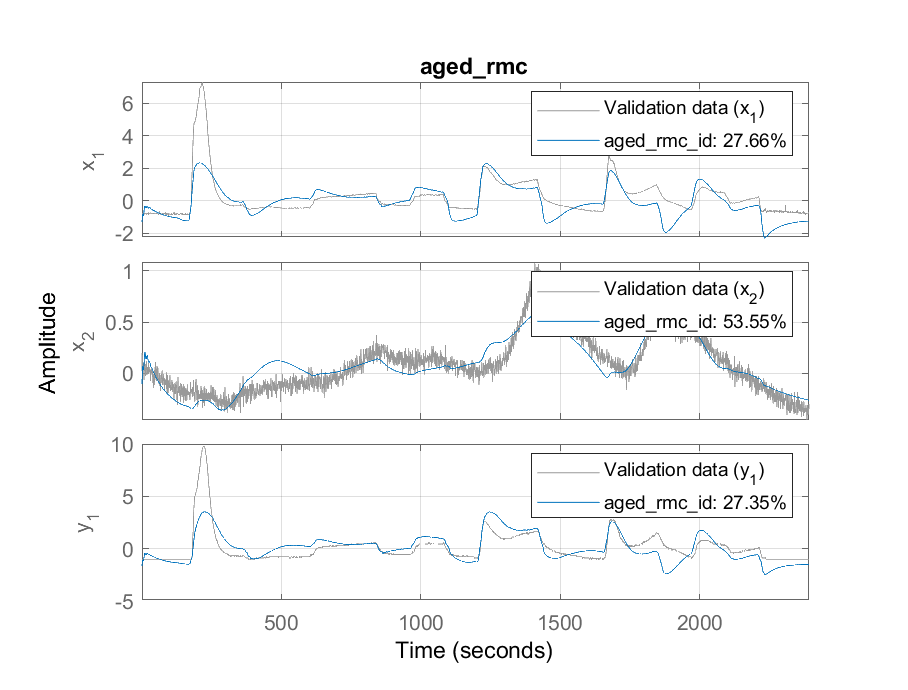
\includegraphics[width=0.7\textwidth]{Part3/figs/4_figs/aged_valid.eps}
    \caption{Comparison of the identified model with the normalized RMC test data for aged catalyst}
    \label{fig:ag_comp}
\end{figure}

Test-cell data (sampled at $5\, Hz$) from three tests (Ramped Mode Cycle (RMC),
hot and cold Federal Test Procedure (FTP))
on both aged and degreened catalysts is used for model structure validation and
model parameter estimation. The validation is done by comparing the test-cell
(experimental) response with the simulation using the estimated model
parameters (Figures~\ref{fig:dg_comp} and \ref{fig:ag_comp}). $\%fit$ is
calculated on the entire time-series of experimental data and simulation to arrive
at the goodness of fit for the model structure. This indicates the percent of
the output data that is captured by the model structure.

As shown in Table~\ref{tab:pfit}, the model structure fits reasonably well
in the cases of RMC and hot FTP data sets. The linear model structure doesn't
capture the dynamics in cold FTP case as the temperature fluctuations are
greater than $\pm 50\, ^0 C$ ($\approx \pm 100\, ^0C$) for which the linear
approximation of the rate constants (\ref{eqn::rate_approx}) is not valid.


\begin{table}[h]
\caption{Model structure validation for test data using prediction error} \label{tab:pfit}
    \begin{center}
    \begin{tabular}{| l | r l | r l |}
        \hline
 & \textbf{Aged} & \textbf{Data} & \textbf{Degreened} & \textbf{Data}
\\
\textbf{Test} & $NO_x$    & $NH_3$    &  $NO_x$   & $NH_3$   \\
& $(\%fit)$ & $(\%fit)$ &  $(\%fit)$& $(\%fit)$\\ \hline
        RMC           & $27.66$ & $53.55$ & $19.98$ & $59.16$ \\ \hline
        hot FTP       & $7.105$ & $38.31$ & $7.385$ & $56$\\ \hline
        cold FTP*      & $23.19$ & $-32.88$& $23.24$ & $-1.77$\\ \hline
\end{tabular}
    \end{center}
\itbf{Note}: $\%fit = 100 \times \lr{1 - \frac{\norm{Y- \hat Y}}{\norm{Y -
mean(Y)}}}$ is the percentage of the measured output that was explained by the
model.\\
*Cold FTP data set is not in the operating range of the linearized model.
\end{table}


The model structure can be further utilized for characterizing catalyst aging
and for diagnostic purposes. Specifically, the values of $N_{12}/\bar x$ could
be a good indicator of the catalyst aging if its value is statistically
different for aged and degreened catalysts. This value for the data sets is
tabulated in Table~\ref{tab:N12_comp}. The statistical validation of
difference in the value of $N_{12}/\bar x$ for aged and degreened catalysts is left for future work.

\begin{table}[h]
\caption{Comparison of $N_{12}/\bar x$ estimate for aged and degreened
    catalysts in test data} \label{tab:N12_comp}
    \centering
    \begin{tabular}{|l|c|c|}
        \hline
        \textbf{Test Data} & \textbf{Aged Data} & \textbf{Degreened Data}\\ \hline
        RMC                & 0.0116        & 0.0034 \\ \hline
        hot FTP            & 0.0099        & 0.0030 \\ \hline
        cold FTP           & -0.0281       & -0.0241 \\ \hline
    \end{tabular}
\end{table}
